% begin module logarithm-def
\begin{frame}
\frametitle{Logarithmic Functions}
\begin{columns}[c]
\column{.3\textwidth}
\ \only<handout:0| -7>{%
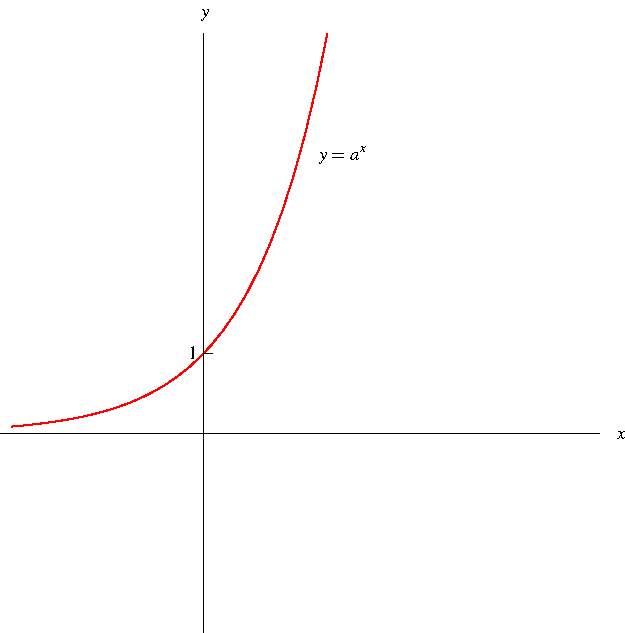
\includegraphics[height=4cm]{logarithms/pictures/07-03-logandexpa.pdf}%
}%
\only<8->{%
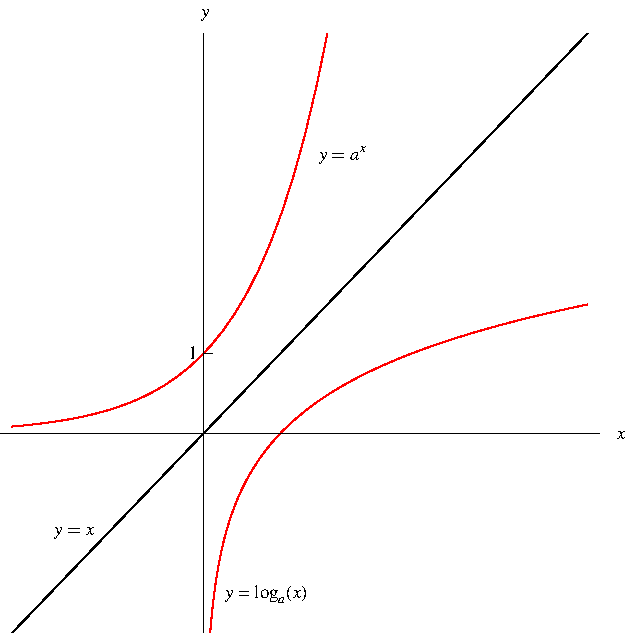
\includegraphics[height=4cm]{logarithms/pictures/07-03-logandexpb.pdf}%
}%
\column{.7\textwidth}
\begin{itemize}
\item  Suppose $a > 0$, $a\neq 1$.
\item<2->  Let $f(x) = a^x$.
\item<3->  Then $f$ is either increasing or decreasing.
\item<4->  Therefore $f$ is one-to-one.
\item<5->  Therefore $f$ has an inverse function, $f^{-1}$.
\item<7->  The graph shows $y = a^x$ for $a > 1$.
\item<8->  The graph of $y = \log_a x$ is the reflection of this in the line $y = x$.
\end{itemize}
\end{columns}
\uncover<6->{%
\begin{definition}[$\log_a x$]
The inverse function of $f(x) = a^x$ is called the logarthmic function with base $a$, and is written $\log_a x$.  It is defined by the formula
\[
\log_a x = y \qquad \Leftrightarrow \qquad a^y = x .
\]
\end{definition}
}%
\end{frame}
% end module logarithm-def
